\documentclass[runningheads]{llncs}
%
\usepackage[T1]{fontenc}
% T1 fonts will be used to generate the final print and online PDFs,
% so please use T1 fonts in your manuscript whenever possible.
% Other font encondings may result in incorrect characters.
%
\usepackage{graphicx}
\usepackage{float}
\usepackage{comment}
% Used for displaying figures. If possible, figure files should
% be included in EPS format.
%
% If you use the hyperref package, please uncomment the following two lines
% to display URLs in blue roman font according to Springer's eBook style:
%\usepackage{color}
%\renewcommand\UrlFont{\color{blue}\rmfamily}
\usepackage{hyperref}
\urlstyle{rm}
%
\begin{document}
%
\title{A Layered Architecture for Digital Twins with Progressive Fidelity: A Case Study in Airport Operations with Specification-First Development}
%
\titlerunning{Digital Twins for Progressive Fidelity}
%
\author{Arthur Chevallier \and German Castignani}
%
\authorrunning{A. Chevallier and G. Castignani}
%
\institute{Luxembourg Institute of Science and Technology\\
\email{arthur.chevallier@list.lu, german.castignani@list.lu}}
%
\maketitle              % typeset the header of the contribution
%
\begin{abstract}
Digital twins of complex cyber-physical systems rarely start at full resolution: they grow from simple representations towards higher spatial, temporal, and behavioural fidelity by integrating physical layouts, real-world data, and decision support. Existing architectures decompose a twin into layers, but do not explicitly govern how fidelity can increase without invalidating existing capabilities. We propose a four-layer architecture in which each layer exposes an explicit contract, so raising fidelity is governed as an extension rather than an implicit rewrite. The topmost layer is decisional, with actions returning to the source system through approval gates. We use a specification-first methodology in which event schemas, data models, and service specifications define the intended boundaries. The architecture is instantiated in VirtualSky International Airport (EVSK), an open-source, ongoing research prototype comprising nine domain services and one API gateway. A repository-history analysis examines the blast radius of four fidelity upgrades, while a conformance audit identifies where specifications alone were insufficient. The case evidence supports append-only inter-layer contracts, backed by contract and regression tests, as a practical principle, while also exposing one lower-layer dependency that remains to be refactored.

\keywords{Digital twins \and Progressive fidelity \and Layered architecture \and Airport operations \and Specification-driven development \and Decision support.}
\end{abstract}
%
%
%
\section{Introduction}\label{sec:introduction}

Digital twins are virtual counterparts of physical systems maintained through structured data flows~\cite{glaessgen2012,grieves2017}. In complex domains such as aviation, they cannot be built at maximum resolution from the outset: data, models, and integrations become available incrementally. A project may begin with a logical event model and later add physical simulation, geospatial representation, live data, analytics, and decision support. Throughout this paper, \emph{fidelity} denotes how closely a twin matches its physical counterpart along spatial, temporal, and behavioural dimensions (Section~\ref{sec:architecture}), thereby supporting more reliable feedback and decision making. Increasing any dimension can alter representations, interfaces, and data flows already used by earlier capabilities. Extension can therefore become restructuring, hindering long-term evolution and reproducibility~\cite{jones2020}.

Existing frameworks provide important decompositions. ISO 23247 defines a manufacturing reference architecture~\cite{iso23247}, Tao et al.\ separate the physical entity, virtual entity, data, services, and connections~\cite{tao2018}, and Redelinghuys et al.\ separate concerns from acquisition to emulation~\cite{redelinghuys2019}. They do not explicitly make \emph{fidelity-preserving evolution} a constraint: higher-fidelity capabilities should extend the contracts of lower layers rather than restructure them. This is the gap investigated here.

We therefore ask:

\begin{quote}
\textbf{RQ1: How can a digital-twin architecture support progressive increases in fidelity while preserving the contracts and functionality of previously implemented layers?}
\end{quote}

We study EVSK, the VirtualSky International Airport digital twin and an ongoing research prototype. Its operational entities and ground truth are synthetic, except for opt-in L2 live ADS-B and METAR feeds. Airports provide a demanding testbed because aircraft, vehicles, passengers, baggage, infrastructure, schedules, weather, and disruptions interact across multiple operational timescales. Existing research provides mature models for individual aspects of this system, including delay propagation~\cite{pyrgiotis2013}, delay cost~\cite{cook2009}, passenger-flow prediction~\cite{ke2017,schultz2019}, and airport digital twins~\cite{conde2024,palasca2025}. EVSK instead uses the airport as an instrument for studying whether progressively richer representations can share stable contracts. Its implementation comprises nine FastAPI domain services behind one API gateway, including a decisional layer for anomaly detection, scenario analysis, optimisation, appraisal, and gated recommendations.

The second question concerns how such an architecture can be implemented and maintained without its contracts eroding. Event schemas, shared concepts, service boundaries, and data flows must remain coherent as a distributed system evolves, and the local correctness of individual changes does not guarantee this. We therefore use a specification-first methodology in which service specifications, event schemas, data models, and simulation rules are defined before implementation and remain authoritative, supplemented by reusable ``skill files'' encoding implementation patterns and known pitfalls. Implementation was assisted by coding agents; we treat this as operational context, and Section~\ref{sec:methodology} delimits where human intervention was required. This motivates:

\begin{quote}
\textbf{RQ2: To what extent does specification-first development preserve architectural contracts during sustained implementation of a progressively evolving digital twin, and where does it require independent verification?}
\end{quote}

The paper makes four contributions:
\begin{enumerate}
\item a layered fidelity architecture that treats progressive, contract-preserving evolution as an explicit architectural principle, with fidelity defined along spatial, temporal, and behavioural dimensions;
\item a specification-first development methodology for maintaining these architectural contracts during implementation;
\item EVSK, a fully open-source airport digital-twin prototype that instantiates the architecture across four layers, including established analytical and ML components used to exercise the layer boundaries; and
\item an empirical examination of the principle, combining an analysis of how changes propagated across layers with an audit of where implementation departed from specification.
\end{enumerate}

The research object is therefore not the act of implementing an airport application, nor a new machine-learning method. It is the architectural principle and its empirical examination; EVSK is the single-case instrument through which contract preservation and violations are observed. The methodology is the engineering discipline used to maintain the principle, together with evidence of where specifications alone were not sufficient.

The remainder of the paper is organised as follows. Section~\ref{sec:related} discusses related work. Section~\ref{sec:architecture} presents the layered fidelity architecture, Section~\ref{sec:methodology} describes the development methodology, and Section~\ref{sec:implementation} presents EVSK. Section~\ref{sec:evaluation} reports the evaluation, followed by discussion and conclusions in Section~\ref{sec:discussion}.


\section{Related Work}\label{sec:related}

Digital-twin research provides several foundations. Kritzinger et al.~\cite{kritzinger2018} distinguish models, shadows, and twins by automated exchange. ISO 23247 specifies manufacturing-domain entities, functional entities, and exchanges~\cite{iso23247}; Tao's five-dimensional model organises physical entity, virtual entity, data, services, and connections~\cite{tao2018}; and three-layer IoT architectures separate perception, network, and application~\cite{sethi2017}. These frameworks permit modular implementation, but do not state backward-compatible fidelity evolution as an invariant. For example, replacing EVSK's weather event with provider-specific METAR fields would force capacity and analysis consumers to change; the cited frameworks locate the affected components but do not forbid that coupling. EVSK instead preserves a canonical event behind an adapter. We compare constraint coverage, not claim that earlier architectures must fail; quantifying them would require comparable longitudinal implementations.

Airport modelling provides the application context for examining this question. Analytical and simulation-based research has addressed delay propagation~\cite{pyrgiotis2013} and the cost of delay~\cite{cook2009}, while machine learning has been applied to passenger-flow and boarding-time prediction~\cite{ke2017,schultz2019}. More recent work explicitly applies digital-twin concepts to airport operations, including turnaround operations~\cite{conde2024}, landside simulation~\cite{palasca2025}, and airport-wide adoption guidance~\cite{acrp2024}. These studies demonstrate the feasibility and value of airport digital twins, but generally address particular operational scopes or fixed capabilities rather than the problem of evolving a twin across fidelity levels without restructuring previously implemented functionality. EVSK uses the domain as a demanding instantiation of the architectural principle rather than as the primary research contribution.

AI-assisted software-engineering studies evaluate repository-level issue resolution~\cite{swebench2024}. We do not evaluate agent performance; RQ2 instead asks whether a specification-first process preserves the contracts introduced by RQ1, and where independent verification remains necessary.

\section{Layered Fidelity Architecture}\label{sec:architecture}

\subsection{Fidelity and why it must be progressive}

We define the \emph{fidelity} of a digital twin along three dimensions: \emph{spatial granularity}, from topological relations between entities to gate-level coordinates and geometry; \emph{temporal resolution}, from discrete simulated events to sub-second live updates; and \emph{behavioural realism}, from discrete state transitions to physically grounded and data-calibrated dynamics. In complex domains such as aviation, a twin cannot be built at maximum resolution from the start. The required data, models, and integrations become available over time, and each must be added to a system that already works. Fidelity is therefore acquired progressively, and the architectural question is whether each increase can be made without restructuring what is already implemented.

\subsection{Four capability layers}

The architecture is a stack of four capability layers, each of which raises fidelity along a different combination of the three dimensions (Table~\ref{tab:fidelity}):

\begin{itemize}
  \item \textbf{L0, logical event-driven simulation.} Domain entities are represented as state machines that communicate purely through events. There is no geometry and no external data at this layer. Something happens, an event records it, and downstream consumers react.
  \item \textbf{L1, physical layer.} Spatial layout is added on top of L0: positions, distances, and the travel or transfer times they induce between entities already defined at L0.
  \item \textbf{L2, geospatial and real-world data layer.} The twin is connected to the outside world. Map-based visualisation, live external feeds, and reference data ground the logical and physical state in observed reality.
  \item \textbf{L3, decisional layer.} Scenario analysis, anomaly detection, optimisation, appraisal, and recommendation are built on the first three layers. Actions reach the source system only through approval gates.
\end{itemize}

\begin{table}[H]
\centering
\caption{Fidelity contribution of each layer along the three dimensions.}
\label{tab:fidelity}
\begin{tabular}{llll}
\hline
Layer & Spatial & Temporal & Behavioural \\
\hline
L0 & topological & discrete events & state transitions \\
L1 & gate-level geometry & unchanged (discrete) & travel and transfer times \\
L2 & georeferenced & live and historical feeds & data-calibrated \\
L3 & asset-level decisions & scenario horizons & prescriptive, gated actions \\
\hline
\end{tabular}
\end{table}

At L3, the spatial gain is not a richer rendering but the ability to target decisions to represented assets, such as a terminal, gate, runway, or flight. Three-dimensional visualisation could increase representational spatial fidelity, but would belong to L1 or L2 unless it formed part of a decision interface; because EVSK does not currently implement it, Table~\ref{tab:fidelity} does not use it as evidence.

Figure~\ref{fig:architecture} summarises this domain-independent stack and shows how its four layers map to the EVSK airport implementation.

\begin{figure}[H]
\centering
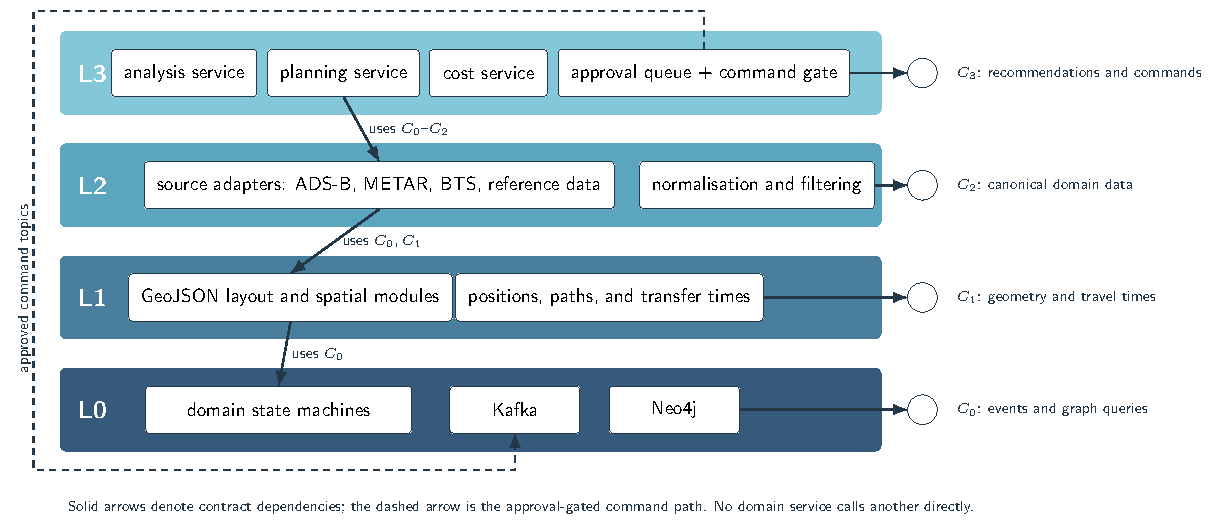
\includegraphics[width=\textwidth]{figures/architecture-components.pdf}
\caption{UML-style component-and-provided-interface view of EVSK's four layers. Solid arrows are dependencies on contracts $C_i$; only the dashed, approval-gated command path closes the loop. Fidelity upgrades may extend a contract but may not alter an existing element.}
\label{fig:architecture}
\end{figure}

L0 to L2 form a digital shadow: data flows from the physical system, or from its simulated stand-in, into the twin~\cite{kritzinger2018}. L3 can close the loop through the command gate. Figure~\ref{fig:architecture} uses standard component and provided-interface idioms to make allowed dependencies reviewable by humans and tools; it is an architectural view, not an executable UML model, and we do not claim that the notation itself improved coding-assistant performance.

A separate axis governs how a single layer matures, independent of which layer it is. Capability within a layer deepens along a fixed ladder, from visualisation, to monitoring and alerting, to prediction, to prescription, to actionability. This ladder describes what a layer \emph{does}, whereas fidelity describes how closely it \emph{represents}; a layer counts as mature once it has climbed the ladder, not merely because it renders something.

\subsection{Contracts and the fidelity-preservation invariant}

Each layer $L_i$ exposes a contract $C_i$ to the layers above it: the event schemas it publishes, the graph model it owns, and the service interfaces it offers. Two rules govern dependencies. A layer may depend on the contracts of lower layers but not on their internals, and lower-layer modules must not import higher-layer internals. Higher layers may influence operational behaviour only through declared lower-layer input or command ports. In particular, L3 may read from L0--L2, while approved actions return through command topics rather than direct imports, keeping the decisional layer removable from the shadow underneath.

These rules yield the architectural invariant on which the rest of the paper rests:

\begin{quote}
\textbf{Fidelity-preservation invariant.} Raising the fidelity of layer $L_i$ may extend its contract $C_i$, but must not modify or remove any existing element of any contract $C_j$. Consequently, layers above $L_i$ continue to operate unchanged.
\end{quote}

For example, replacing synthetic weather with a live METAR feed changes the implementation of an L2 adapter, but the events that L3 consumes keep the same schema. Upgrading a layer's fidelity thus changes that layer's modules and, at most, adds to its contract, and it does not trigger refactoring in the layers that consume it. Section~\ref{sec:evaluation} tests this property against the development history of EVSK.

\subsection{The L2 to L3 boundary and current approval gate}

Because L3 can trigger actions, corrupted data crossing from L2 is consequential. EVSK currently applies source-specific parsing and filtering in its adapters (including required-position and radius checks for ADS-B), canonical envelope construction for Kafka events, Pydantic validation at REST boundaries, and event-ID deduplication in consumers. These checks reduce malformed and duplicate input, but they are not a single end-to-end integrity gate: there is no runtime schema-registry validation, uniform plausibility policy, or source provenance score across all feeds. Moreover, the prototype planning-model trainer reads the BTS extract directly rather than through the planning adapter. We therefore exclude those prototype predictors and their scores from the evaluation and treat adapter-only ingestion plus runtime schema validation as future hardening.

The approval gate is a bounded prototype, not a complete safety case. It blocks configured actions, skips low-confidence ones, auto-approves eligible actions, and holds safety-guarded actions for an approver role. Only concrete supported mappings---currently flight holds and gate reassignments---produce domain commands; aggregate recommendations remain audit records and the queue is in memory. Durable proposals, broader mappings, calibrated confidence and provenance, and stronger policy separation remain future work.

\subsection{Generality}

What the architecture fixes is the order in which fidelity is added and the contracts between layers, not the domain those layers describe. A hospital campus twin could follow the same order: patient, staff, and equipment state machines on an event bus at the base, ward and building layout above, real-time location and environmental sensing next, and bed-allocation or staffing optimisation at the top. The same layering applies to smart ports, manufacturing plants, and urban mobility networks. We use an airport, EVSK, as the concrete instantiation and stress test in the remainder of the paper.

Section~\ref{sec:implementation} shows how EVSK realises each layer with a concrete technology stack, together with the architectural invariants that keep them composable in practice.

\section{Enforcing Layer Contracts with Specification-First Development}\label{sec:methodology}

The layered architecture in Section~\ref{sec:architecture} keeps fidelity additions from forcing a rewrite by fixing what each layer may depend on. That guarantee holds only if the implementation actually respects those contracts, and nothing about the architecture enforces that on its own. The methodology that keeps the two aligned rests on an inversion of the usual workflow: the specification is written first, is machine-readable, and is authoritative. Implementation may not deviate from it, and where reality demands a change, the spec is updated first and the code follows. Before any service is implemented, four definitions already exist: the event-bus schemas, the graph data model, the simulation rules, and one specification per service describing its endpoints, events, state machines, and ownership boundaries. Each new layer, in practice, starts as a specification of the contract it will expose to the layer above and consume from the layer below, before a single line of that layer's code is written.

This discipline has an intellectual lineage older than coding assistants. Writing the authoritative description before the implementation echoes formal specification traditions~\cite{lamport2002}, and decomposing the system so that each service hides exactly one set of design decisions follows Parnas' information-hiding criteria~\cite{parnas1972}. Because the specifications are machine-readable, they can also serve as the context for automated coding assistance, which made drift between specification and code more costly than in a purely manual workflow.

Complementing the per-service and per-layer specifications are ``skill files'', which encode reusable project knowledge in a form readable by both humans and coding assistants. Each skill file has three parts: concept explanation, copy-paste patterns, and gotchas. The patterns keep new code consistent with the project's idioms, and the gotchas encode failures that review caught the hard way, so the same mistake is not repeated. Cross-cutting skills exist for exactly the four runtime invariants of EVSK (Section~\ref{sec:implementation}): the simulation clock, the event bus, the graph as single source of truth, and the no-silent-mutation rule. These are the invariants most likely to be violated under time pressure, since violating any one of them is often the fastest way to make a feature appear to work. Each service additionally owns one skill file documenting its own state machines and quirks.

Entry-point files (\texttt{CLAUDE.md}, \texttt{AGENTS.md}, and editor rule files) instruct the assistant to load the relevant specification and skill file before writing code. Hard rules act as guardrails, and each one maps directly onto a layer contract rather than a general best practice: no wall-clock time in business logic, no service-to-service HTTP calls, no silent mutations, and all operational entities and ground truth synthetic except opt-in L2 live feeds. Because each rule corresponds to a specific invariant, a violation is detectable by search or contract test, rather than surfacing later as a layer-boundary failure that looks unrelated to its cause.

\paragraph{Role of coding assistants and the human perimeter.}
EVSK was implemented with the help of AI coding assistants operating inside this specification framework. We treat this as operational context and not as a contribution, and we delimit it precisely. The assistants produced code within the boundaries set by the specifications. Humans were responsible for everything that defines those boundaries: writing and approving the specifications and event contracts, deciding the hard rules, and reviewing every change against the layer contracts. Human intervention was also required to correct assistant output that satisfied the immediate task but not the architecture. A mid-project audit (Section~\ref{sec:discussion}) found three such cases: duplicated constants that had diverged, recommendations that were never connected to command topics, and an ML endpoint that reported success without having trained a model. In each case the code conformed to a local reading of the task but not to the contract, and the fix was made by a human reviewer and, where relevant, promoted into a skill file as a gotcha.

Periodic post-mortems close the loop: defects and near-misses found in review, including layer-boundary violations that slipped past the hard rules, are promoted back into skill files, so the knowledge base accumulates detail where an added layer most recently threatened the contract beneath it. Progressive fidelity therefore has to be achieved twice: once in what the twin models, and again in how faithfully the implementation matches what was specified.

\section{EVSK: Instantiating the Layered Architecture}\label{sec:implementation}

EVSK instantiates the architecture as nine FastAPI domain services behind a thin Node.js/Express API gateway, with React/TypeScript dashboards, Kafka as the event backbone~\cite{kreps2011}, Neo4j as the graph store~\cite{angles2008}, an observability stack, and staged CI. The conventional stack keeps the evaluation focused on the architectural claim rather than on a novel platform.

Each layer is realised with a concrete slice of this stack. L0 uses Kafka and Neo4j for the domain state machines. L1 adds terminal, gate, runway, and taxiway geometry. L2 adds map visualisation, an ADS-B overlay, live and historical METAR weather, BTS schedule calibration, and OurAirports/OpenFlights reference data. L3 adds what-if and Monte-Carlo scenario analysis, anomaly detection, recommendations, and discounted-cash-flow investment appraisal on Eurocontrol Standard Inputs~\cite{eurocontrol2024}. The planning service also contains demand and delay predictors, but their present training pipeline is a prototype: the demand feature set leaks its target and the delay labels are rule-derived. We report neither their error nor discrimination as evidence of predictive skill.

Four runtime invariants are intended to keep these layers composable. Services use the simulation clock rather than wall-clock time for business logic; a single orchestrator broadcasts ticks on a dedicated topic (see Annex, Fig.~\ref{fig:clock}). EVSK can run at configurable speed up to $3600\times$ real time and supports deterministic replay when fixtures, seeds, and event order are held fixed. Operational event topics carry facts, while commands use separate topics. The graph store is the source of truth for structural state, each service owns its node labels, and in-memory caches are intended to be rebuildable after restart. The no-silent-mutation rule requires modelled state changes to emit events. These are conformance targets checked by review and tests, not guarantees supplied by the technology stack.

EVSK's build history provides case evidence for this composability: the system moved from pure simulation, through map and live-data integration, to scenario analysis and financial planning without re-platforming the stack. Section~\ref{sec:evaluation} audits the stronger contract-isolation claim and reports where it did not fully hold.

Domain depth is where the implementation earns the word ``twin''. The flight domain runs a nine-state lifecycle state machine with runway queueing and delay cascades that propagate up to five hops, mirroring network-level propagation models~\cite{pyrgiotis2013} (see Annex, Fig.~\ref{fig:flight-lifecycle}). Passenger flow contains a LightGBM model that predicts security-queue depth ninety minutes ahead~\cite{ke2017,schultz2019}. We classify this predictor as an embedded L0 component: on each simulation tick its output enters the security-throughput calculation, changing how many passengers transition from the security queue to airside. The write-back is therefore an internal, event-emitting L0 feedback loop, not a dependency from L0 on L3. Baggage travels a thirty-zone conveyor network with dangerous-goods screening, and weather is a four-state finite-state machine whose runway-capacity impacts cascade into the flight domain (see Annex, Fig.~\ref{fig:weather-cascade}). A rule-based incident engine cascades five hazard types through the graph under explicit depth limits.

The twin is open at its configuration and data boundaries. Airport identity, terminals, gates, runways, operational constants, and cascade limits are loaded from YAML rather than embedded in service logic. A shared registry supplies a common adapter protocol in the simulation orchestrator, weather service, and passenger service; the planning service uses a separate local adapter factory. Within those three adopters, a source can be switched without changing its downstream consumer. The scoped Open/Closed claim is therefore that configuration and adapters extend the represented world while tested domain logic remains unchanged.

The simulated day is operationally plausible at scale: 420 flight movements, roughly 30{,}000 passengers, and roughly 36{,}000 baggage items, driven by the simulation clock described above.

The decisional layer is implemented as part of the current research prototype. The cost service maintains profit-and-loss statements, EC~261/2004 liability~\cite{eu261}, and carbon accounting. The planning service runs a Monte-Carlo infrastructure scenario engine producing NPV, IRR, and payback appraisals. The analysis service provides Isolation-Forest anomaly detection, slot-allocation MILP, and recommendations routed through the approval queue. Concrete supported actions use command topics; other recommendations are presently audit-only, so command coverage remains incomplete.

To support reproducibility, specifications, skill files, infrastructure definitions, data pipelines, and the implementation are available in the \href{https://github.com/arthur-chevallier/airport-digital-twin}{project repository}. Airport identity and much of the operational structure are configuration-driven; adapting EVSK to another airport is intended to require configuration and adapter changes rather than a separate codebase, although this has not yet been validated in a second deployment.

\section{EVSK: Evaluation of progressive fidelity in our use-case}\label{sec:evaluation}

This section examines progressive fidelity in EVSK. Because the repository has no prospective milestone ledger, this is a retrospective path-level case analysis rather than a controlled benchmark.

\subsection{Audit design}

The unit of analysis is an upgrade path, not a raw commit count. We traced L1 geometry, L2 live feeds, BTS-based calibration, and L3 cost analysis from their introducing diffs to the current implementation, specifications, schemas, and tests. The reproduction script \texttt{blast\_radius\_metrics.py} applies declared path scopes to the introducing changesets and uses Git's diff tree to count unique files, pre-existing files modified, and top-level components touched. The counts complement the contract audit and describe change spread, not productivity.

\begin{figure}[H]
\centering
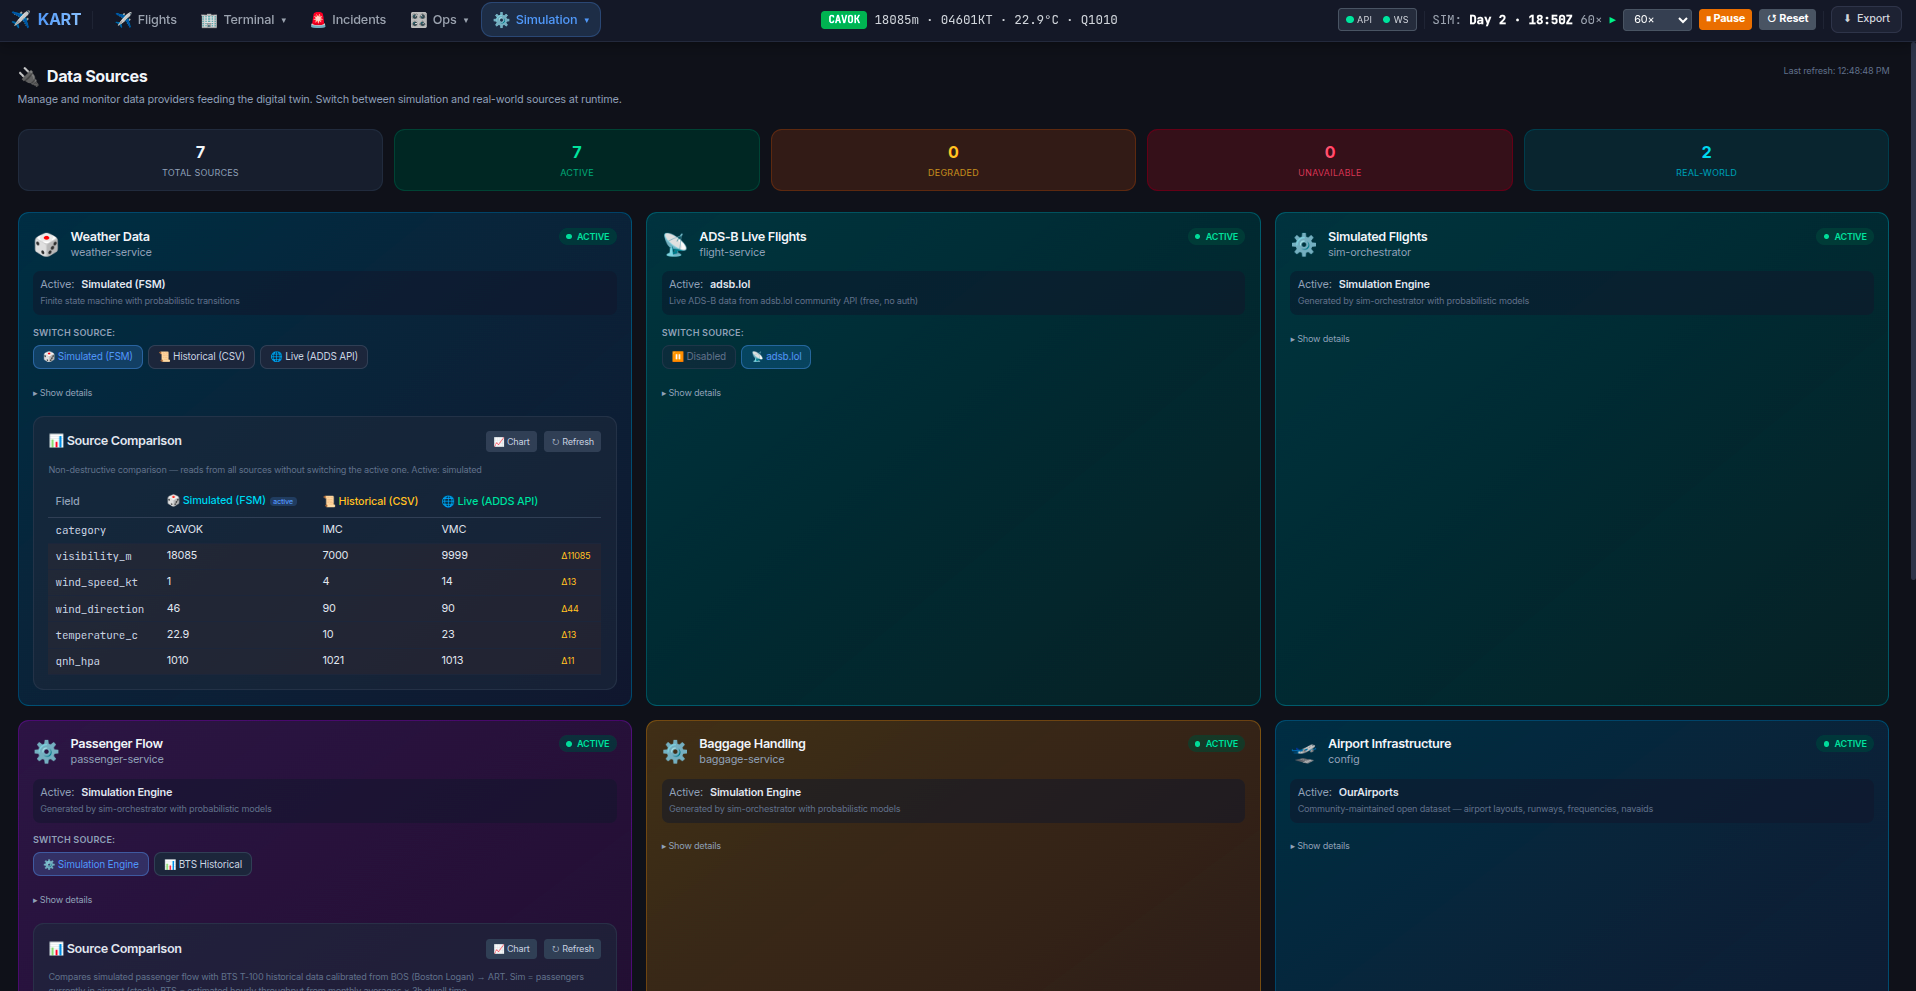
\includegraphics[width=.63\textwidth]{figures/data-sources-dashboard.png}
\caption{L2 implementation view used in the audit: the source-selection dashboard. The shared registry is used by the simulation orchestrator, weather service, and passenger service; planning adapters use a separate local factory.}
\label{fig:datasources}
\end{figure}

\subsection{Results across upgrade paths}

Figure~\ref{fig:datasources} shows the L2 source-selection surface; the L0 graph and L3 cost views are retained in the Annex (Figs.~\ref{fig:neo4j} and~\ref{fig:cost}). Table~\ref{tab:upgrades} reports what changed underneath them. The automated radii---unique scoped files / pre-existing files modified / components touched---are 14/6/5 for L1 geometry, 17/9/7 for L2 live feeds, 7/5/3 for BTS calibration, and 35/12/6 for L3 cost analysis.

\begin{table}[t]
\centering
\small
\caption{Observed contract and consumer effects of four fidelity upgrades.}
\label{tab:upgrades}
\begin{tabular}{p{.19\textwidth}p{.34\textwidth}p{.35\textwidth}}
\hline
Upgrade & Touched subsystem & Contract and consumer effect \\
\hline
L1 geometry & Layout fixture, spatial utilities, domain transitions & Added geometry; L0 contracts unchanged \\
L2 live feeds & ADS-B/weather adapters and source UI & Existing domain representations; consumers unchanged \\
Data calibration & BTS parser, schedule and passenger generators & Contracts unchanged; L0 internals edited \\
L3 cost analysis & New consumer, persistence, API, dashboard & New cost contract; existing payloads unchanged \\
\hline
\end{tabular}
\end{table}

L1 geometry and L2 live feeds added geometry, adapters, and presentation components while retaining operational event shapes. L3 cost analysis added persistence, an API, and a dashboard, but remained interface-additive: it consumed existing facts and published a new contract without changing an existing producer or consumer.

The BTS path is a counterexample to strict implementation isolation. External contracts stayed stable, but calibration added imports and branches inside the L0 schedule and passenger generators. It preserved consumer compatibility while editing lower-layer code; a cleaner design would materialise calibrated configuration through a declared L0 input port. Thus the audit supports preservation of existing contract elements, not the stronger claim that fidelity upgrades never edit lower-layer code.

\subsection{Specification conformance}

Event-bus and data-model specifications changed with the cost and command-topic code. Contract tests cover envelopes and handoffs; fidelity tests exercise runway and investment assumptions; approval tests cover classification, transitions, and supported commands. They do not establish source truthfulness, end-to-end availability, or autonomous-operation safety, so the BTS dependency and earlier audit findings still require code inspection.

\section{Discussion and Conclusion}\label{sec:discussion}

The results address the two research questions directly. \textbf{RQ1} asked whether fidelity can be increased while preserving previously implemented layers. All four audited paths preserved existing event and service contracts, and no existing consumer required an interface migration. Three paths were additive at both the interface and module levels; BTS calibration edited lower-layer generators and therefore exposes a conformance gap. The supported conclusion is consequently about contract preservation, not zero change to lower-layer implementation.

\textbf{RQ2} asked whether specification-first development can preserve these contracts during sustained implementation, and where it requires independent verification. The experience was useful but insufficient on its own. A mid-project audit found diverging duplicated constants, recommendations disconnected from command topics, and an ML endpoint that reported success without training a model. Cross-service contract tests now check event-envelope fields and producer/consumer handoffs, while fidelity regression tests exercise planning assumptions. These executable checks and periodic audits are necessary complements to the specifications.

The findings are complementary: \emph{the architecture defines what must remain stable; the methodology helps preserve it}. Neither is sufficient alone. Contracts, specifications, executable checks, and dependency audits must operate together. Existing reference architectures could adopt the same invariant; EVSK's distinction is to state it as a rule and audit concrete upgrade paths against it.

Ports, hospitals, and warehouses could use the same ordering of event state, spatial representation, observed data, and decisions. Transfer remains a proposition: this is one retrospective case, one small team, and synthetic ground truth~\cite{runeson2009}. We did not reimplement EVSK under ISO 23247, Tao's model, or a three-tier IoT architecture. Comparative superiority, productivity effects, and defect-rate improvements therefore cannot be inferred.

Future work will invert the BTS calibration dependency, persist approval proposals, extend command-topic coverage, add runtime schema and provenance validation, and test the architecture in a second domain or federated multi-airport setting. Overall, EVSK provides qualified support for \textbf{RQ1} at the contract level and supports \textbf{RQ2} by showing that specification-first development helps maintain boundaries but requires independent verification.

\noindent\textbf{Acknowledgments and use of AI.} No specific funding was received. AI tools assisted language editing; the authors remain responsible for the content.

% ---- Bibliography (excluded from the 12-page main-text limit) ----
\clearpage
\bibliographystyle{splncs03_unsrt}
\bibliography{refs.bib}

\newpage
\section*{Annex}

\begin{figure}[H]
\centering
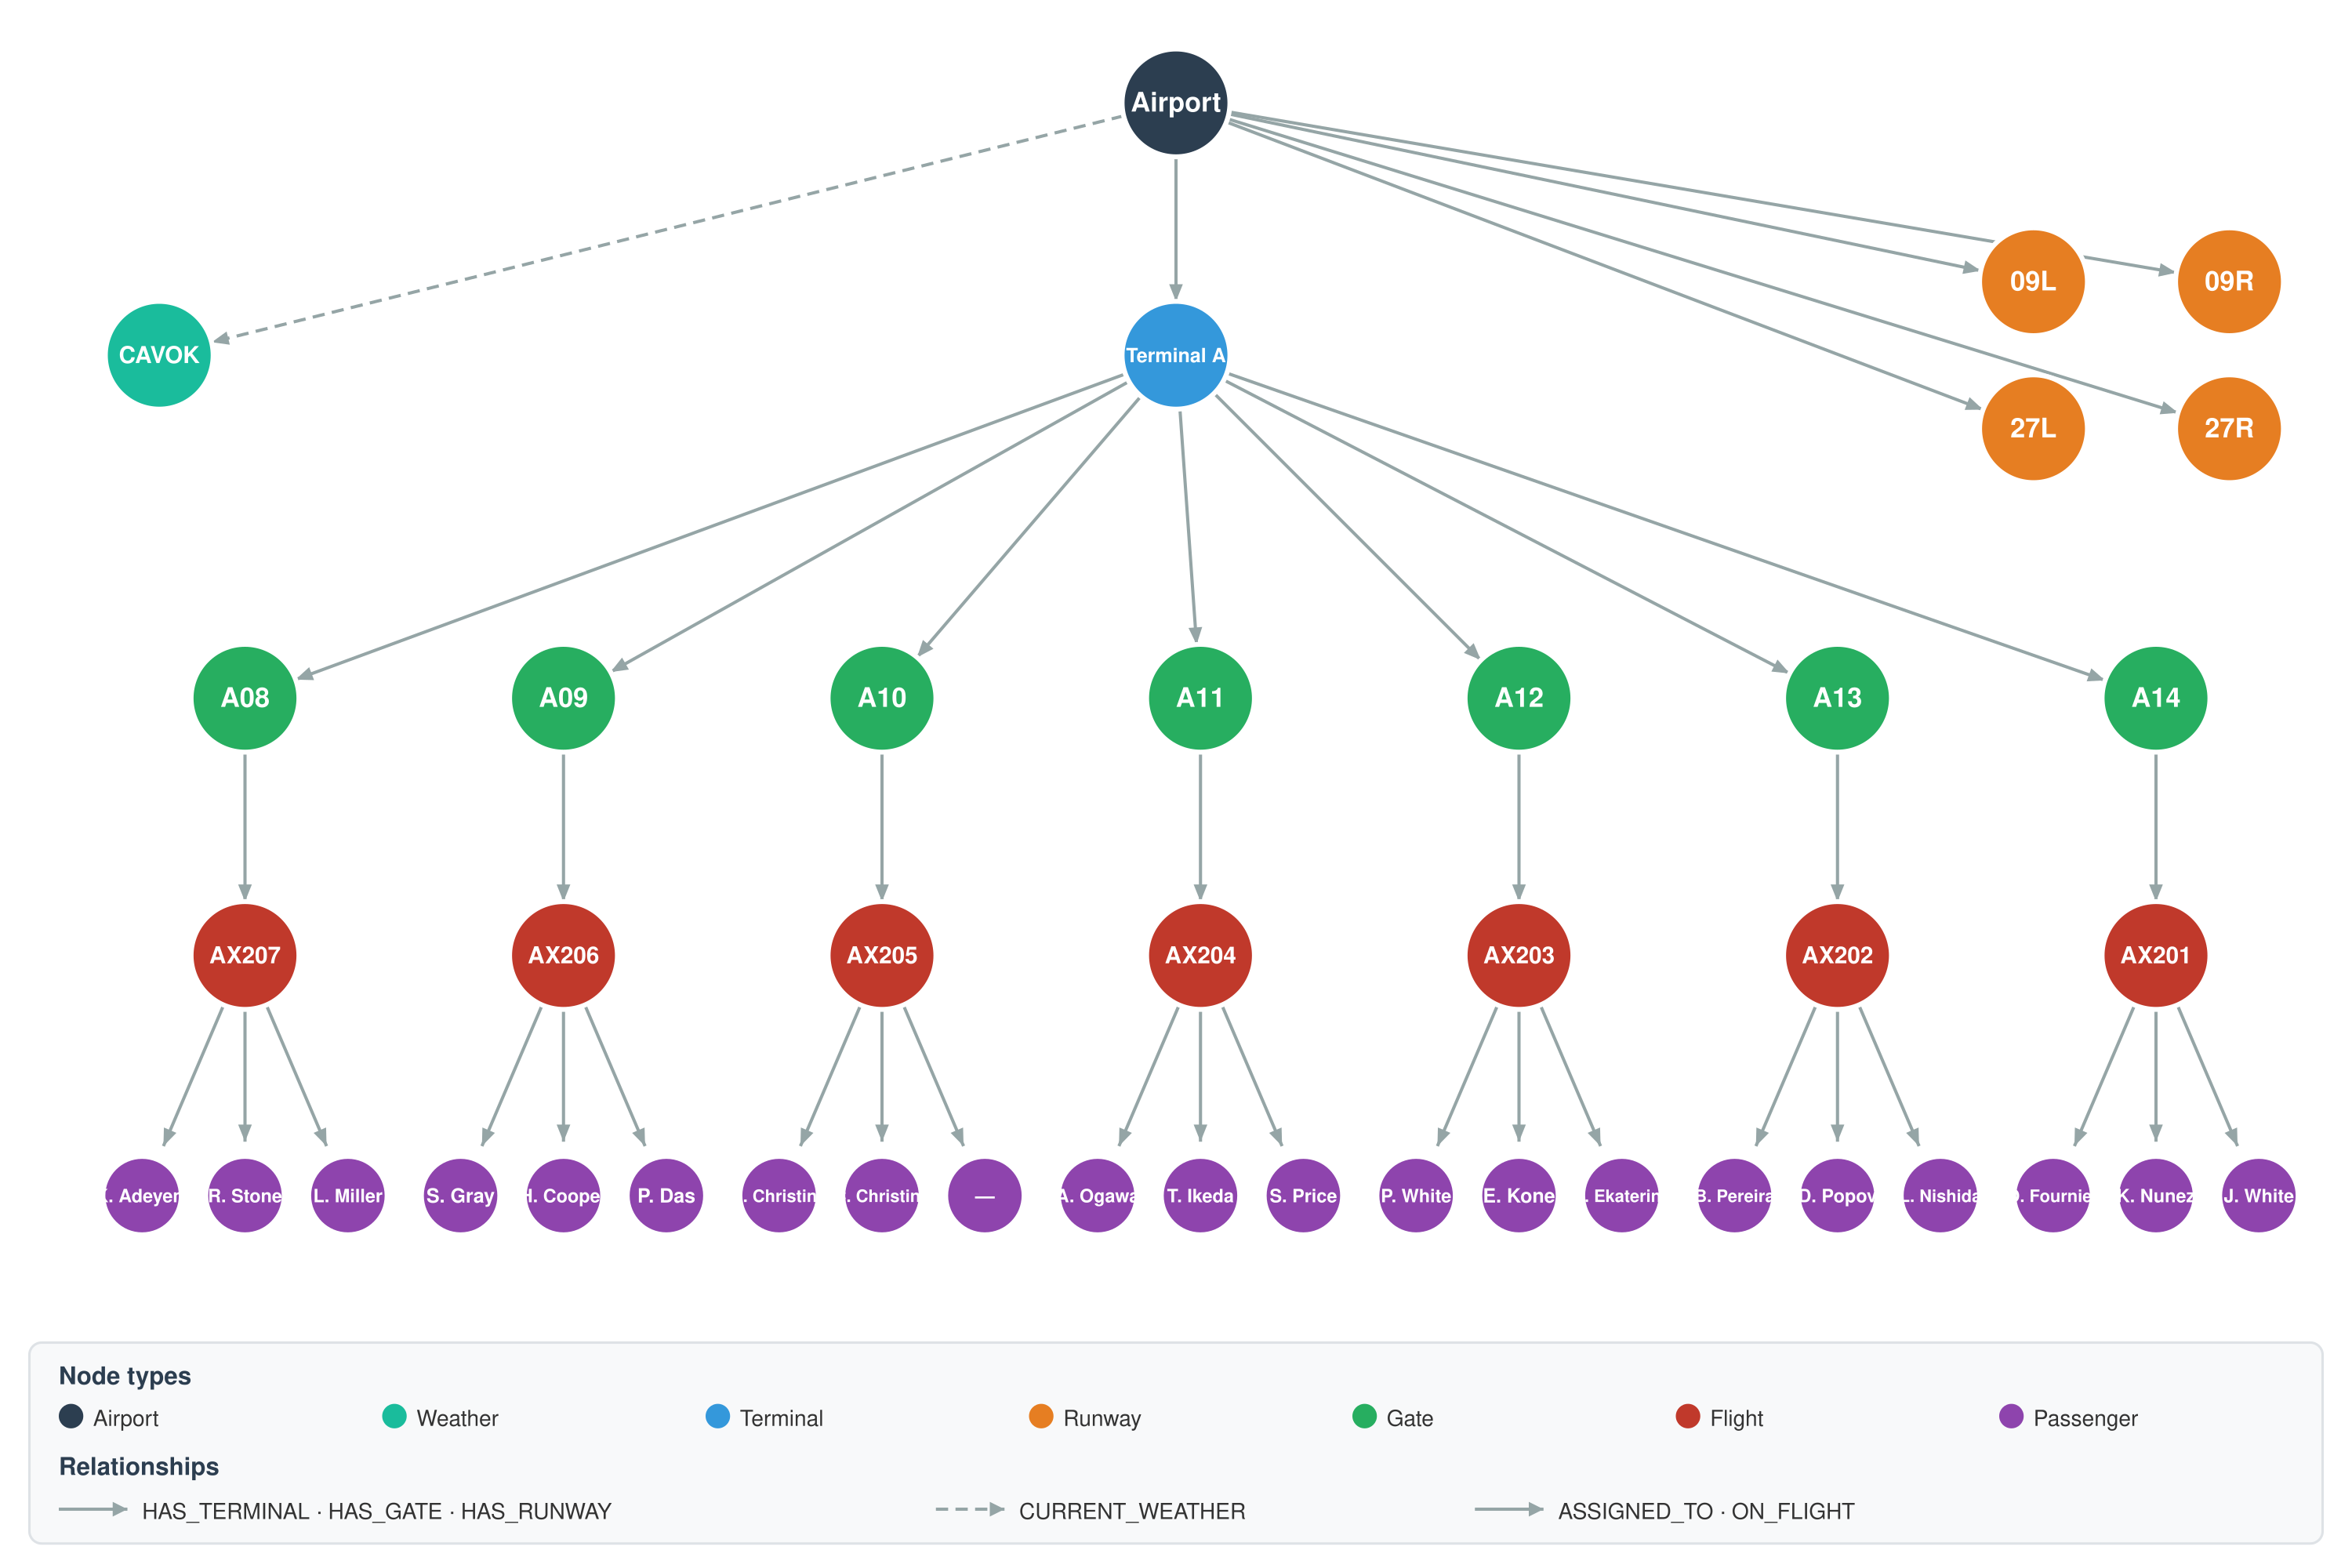
\includegraphics[width=\textwidth]{figures/visualisation.png}
\caption{L0 implementation view: Neo4j stores the operational graph reconstructed from domain events.}
\label{fig:neo4j}
\end{figure}

\begin{figure}[H]
\centering
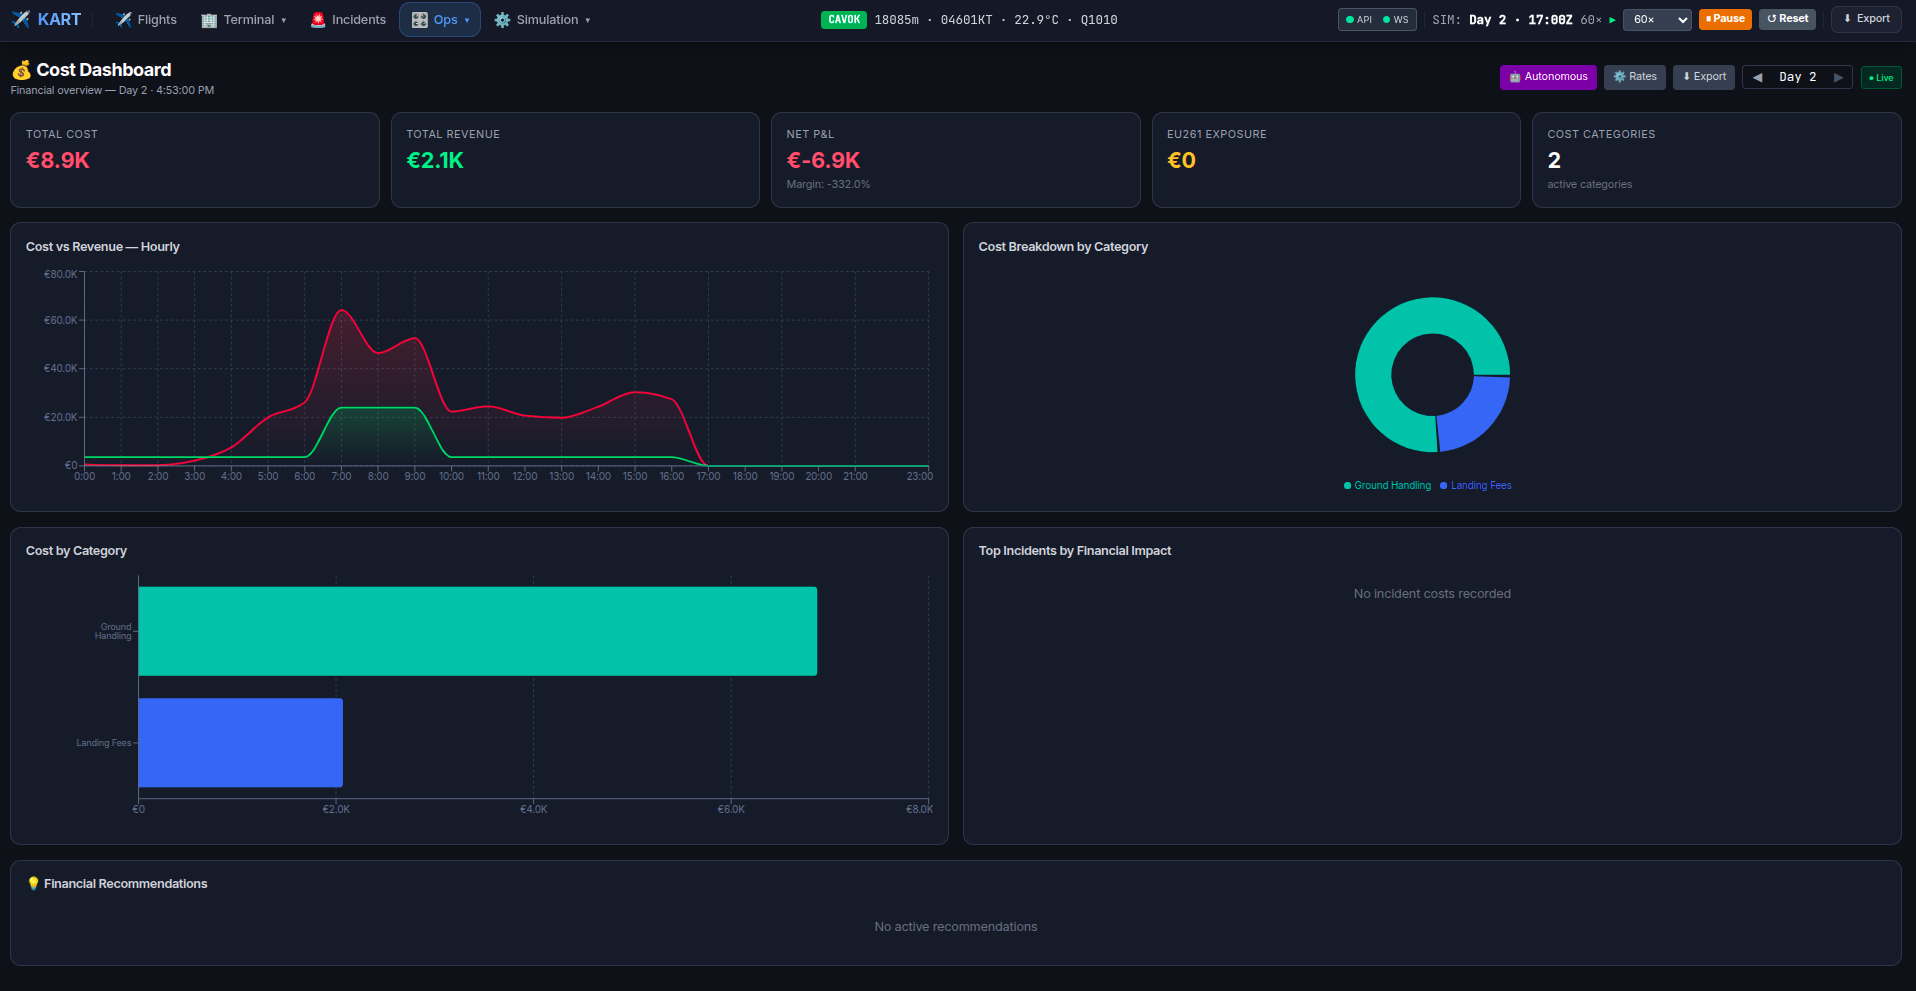
\includegraphics[width=\textwidth]{figures/cost-dashboard.png}
\caption{L3 implementation view: the cost dashboard consumes operational events to present profit-and-loss and cost categories.}
\label{fig:cost}
\end{figure}

\begin{figure}[H]
\centering
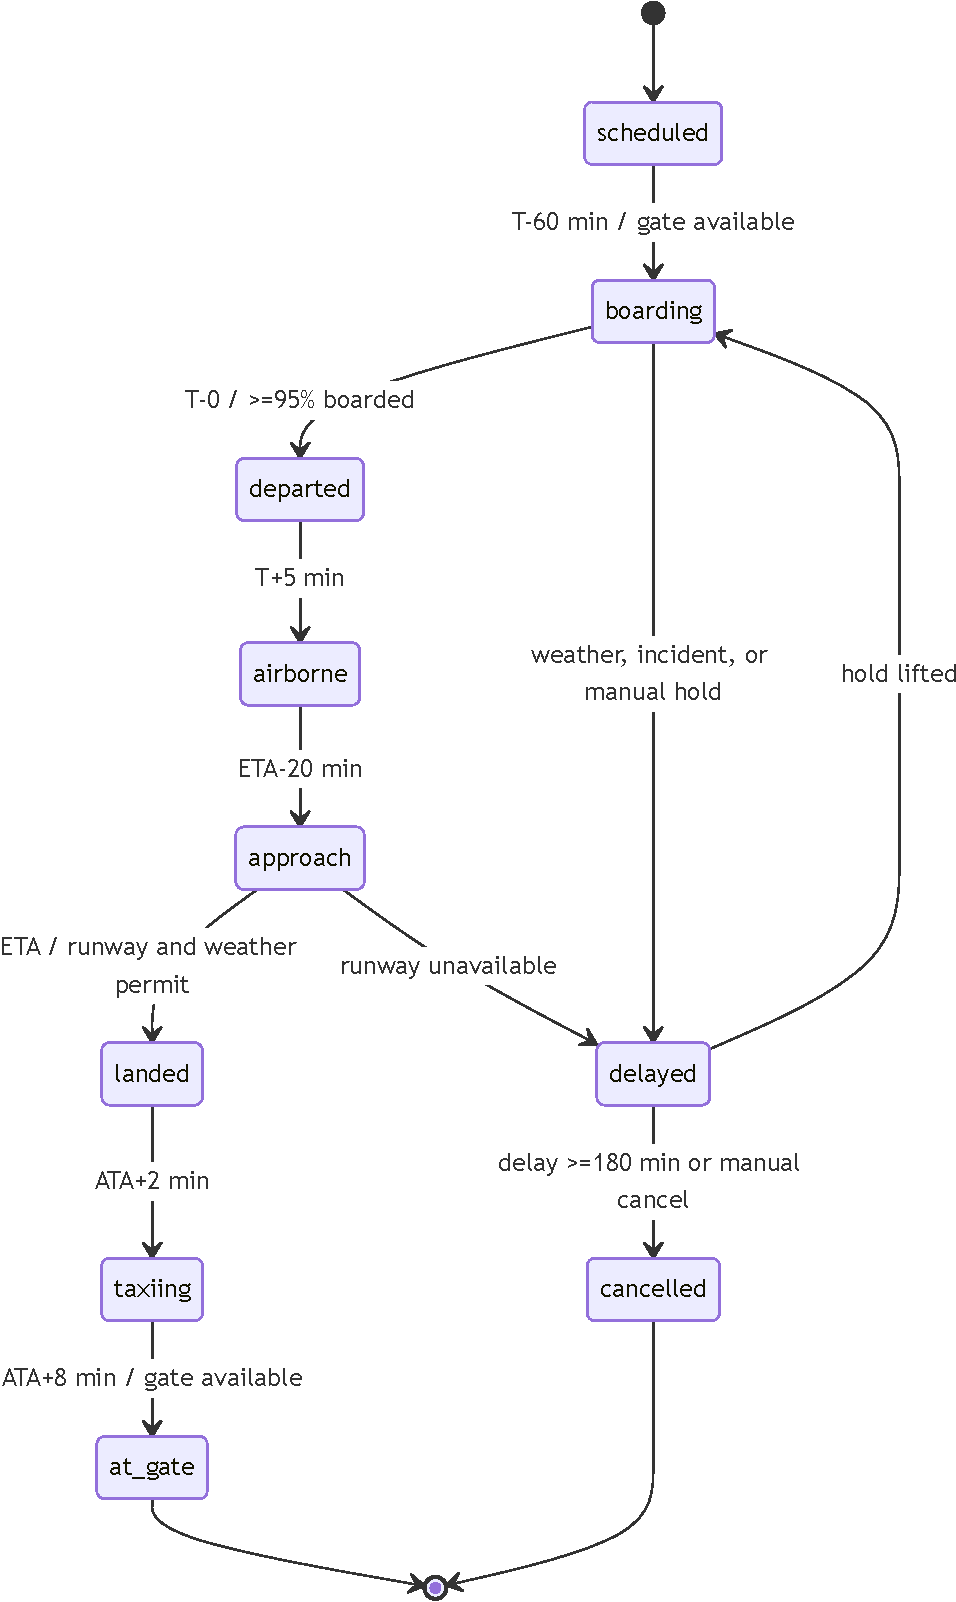
\includegraphics[height=.75\textheight,keepaspectratio]{figures/flight-lifecycle.pdf}
\caption{Flight lifecycle driven by simulated time and constrained by gates, runways, weather, incidents, and boarding progress.}
\label{fig:flight-lifecycle}
\end{figure}

\begin{figure}[H]
\centering
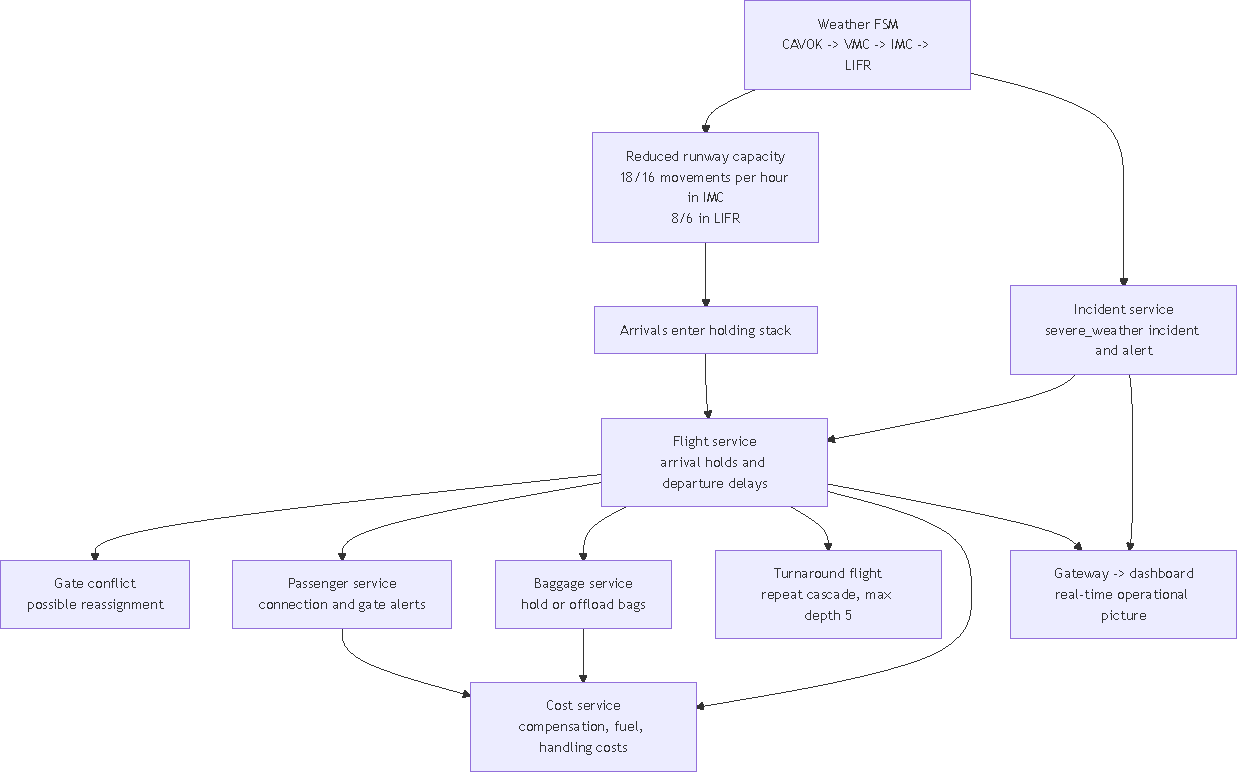
\includegraphics[width=\textwidth]{figures/weather-cascade.pdf}
\caption{Causal propagation from weather degradation to runway capacity, flight delays, passenger and baggage disruption, and operational cost.}
\label{fig:weather-cascade}
\end{figure}

\begin{figure}[H]
\centering
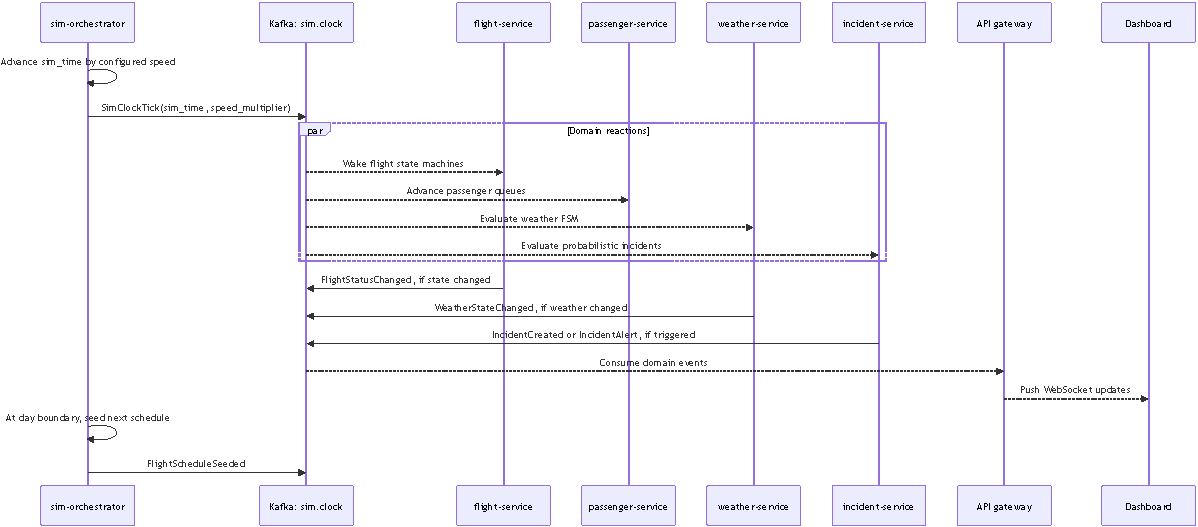
\includegraphics[width=\textwidth]{figures/clock.pdf}
\caption{Simulation-clock coordination in EVSK. A single virtual-time stream drives every service, and resulting facts are pushed to the dashboard through the gateway.}
\label{fig:clock}
\end{figure}

\end{document}
